%%%%%%%%%%%%%%%%%%%%%%%%%%%%%%%%%%%%
% Header                           %
%%%%%%%%%%%%%%%%%%%%%%%%%%%%%%%%%%%%
% 
% Revisions: 2017-04-10 Martin R�del <martin.raedel@dlr.de>
%                       Initial draft
%               
% Contact:   Martin R�del,  martin.raedel@dlr.de
%            DLR Composite Structures and Adaptive Systems
%          
%                                 __/|__
%                                /_/_/_/  
%            www.dlr.de/fa/en      |/ DLR
% 
%%%%%%%%%%%%%%%%%%%%%%%%%%%%%%%%%%%%
% Content                          %
%%%%%%%%%%%%%%%%%%%%%%%%%%%%%%%%%%%%

\levelstay{Selection}
\label{sec:Use_ParaView_Selection}

\leveldown{Create a selection}
\label{sec:Use_ParaView_Selection_Create}

Selections are

\begin{itemize}[noitemsep]
  \item a mechanism to identify subset of a dataset
  \item Focus on selected subset:
  \begin{itemize}[noitemsep]
    \item Inspect properties of the subset
    \item Further process subset alone
  \end{itemize}
  \item Track subset over time
\end{itemize}

Selections are performed in a toolbar in the RenderView. At first it has to be chosen if the items should be added to or removed from the selection using the following buttons:

\begin{tabularx}{\linewidth}{clXclXcl}
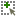
\includegraphics[width=\iconsize]{Figures/Icons/pqSelectPlus16}	& Add selection	&&
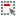
\includegraphics[width=\iconsize]{Figures/Icons/pqSelectMinus16}	& Subtract selection	&&
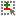
\includegraphics[width=\iconsize]{Figures/Icons/pqSelectToggle16}	& Toggle selection
\end{tabularx}

In a second step the kind of item, cells or points, to be selected has to be specified:

\begin{tabularx}{\linewidth}{lXclXcl}
Points: &&
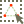
\includegraphics[width=\iconsize]{Figures/Icons/pqSurfaceSelectionPoint24}	& Select points on	&&

\includegraphics[width=\iconsize]{Figures/Icons/pqFrustumSelectionPoint24}	& Select points through	\\
&&
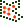
\includegraphics[width=\iconsize]{Figures/Icons/pqPolygonSelectSurfacePoint24}	& Select points with polygon	&&
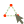
\includegraphics[width=\iconsize]{Figures/Icons/pqSurfaceSelectionPointInteractive}	& Select points interactive	\\
% 
Cells: &&
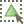
\includegraphics[width=\iconsize]{Figures/Icons/pqSurfaceSelectionCell24}	& Select cells on	&&

\includegraphics[width=\iconsize]{Figures/Icons/pqFrustumSelectionCell24}	& Select cells through	\\
&&
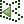
\includegraphics[width=\iconsize]{Figures/Icons/pqPolygonSelectSurfaceCell24.png}	& Select cells with polygon	&&
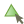
\includegraphics[width=\iconsize]{Figures/Icons/pqSurfaceSelectionCellInteractive}	& Select cells interactive
\end{tabularx}

Selection steps can be repeated as long as no Filter dependent on the selection is active. The currently selected entities are highlighted.

\levelstay{Limit display to selection}
\label{sec:Use_ParaView_Selection_LimitTo}

To limit the model to a user defined selection:

\begin{enumerate}[noitemsep]
\item Import result file to \marktool{\paraviewname}
\item Create a selection
\item From the menu bar:
  \begin{itemize}[noitemsep]
  \item Click Filters
  \item Click Data Analysis
  \item Click \textit{Extract Selection}
  \end{itemize}
  or click 
\includegraphics[width=\iconsize]{Figures/Icons/pqExtractSelection24} in the Data Analysis toolbar
\item Click \textit{Apply} in the newly opened Properties tab
\end{enumerate}

\levelstay{Remarks}

\begin{enumerate}[noitemsep]
   \item  Selected points lie in a virtual box. If the deformation of the model are to big, the points move outside the box and the allocation is lost. This might be an issue for plotting data. This can be solved by setting the deformation scaling to zero.
\end{enumerate}
